\cleardoublepage
\chapter{基于LSH树的验证机制}
\label{sec:lsh}
从本文的测量数据中可以分析出,在传输的数据中,数据完整性证明几乎占据了一半的比例。
这些证明通常以默克尔树的形式组织,由一连串的哈希值构成。
在默克尔树结构中,非叶子节点的哈希数量与原始数据点的数量大致相同。
鉴于物联网数据单元的大小与哈希值相近,这意味着为了验证数据的完整性,需要传输的数据量几乎是原始数据量的两倍。
在数据传输过程中,如何减少完整性证明大小,成为了一个亟待解决的难题。

\section{LSH树结构与工作流程}

\begin{figure}[t]
    \centering
    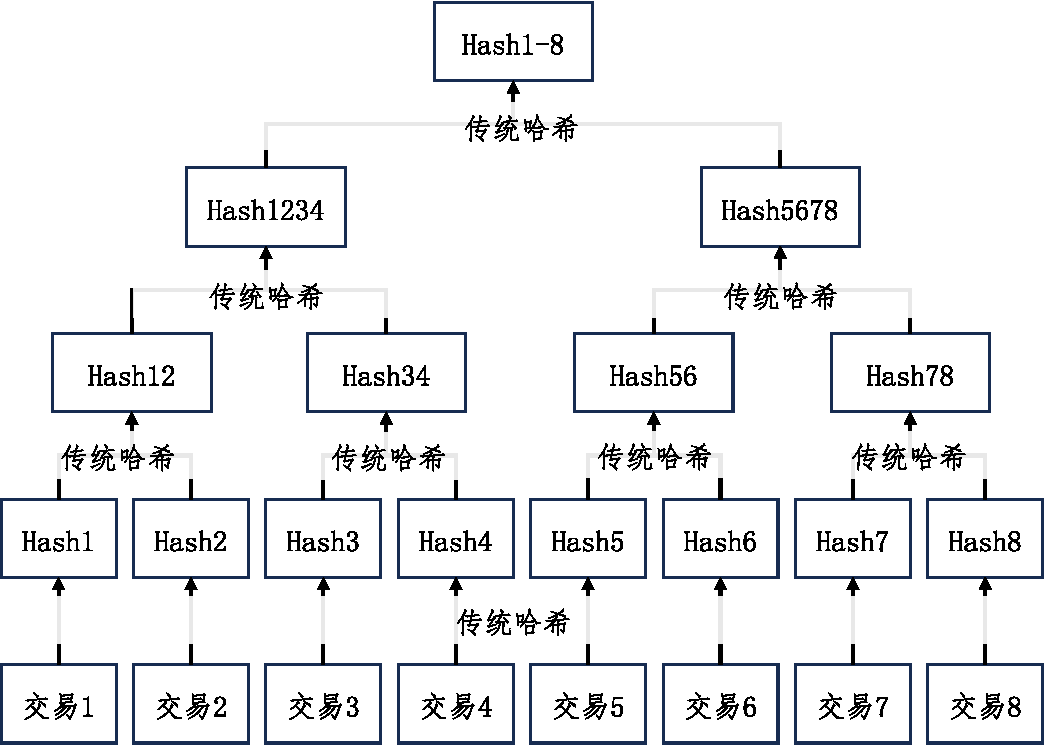
\includegraphics[width=0.85\linewidth]{figures/timechain/merkle.pdf}
    \caption{默克尔树的结构}
    \label{fig:merkle}
\end{figure}

默克尔树(Merkle Tree)作为一种轻量级的完整性验证机制,在许多区块链平台中广泛使用。
如\autoref{fig:merkle}所示,默克尔树是一种二叉树结构,其中每个非叶节点都是其两个子节点的哈希值。
具体来说,叶节点通常包含底层交易的哈希值,而非叶节点则包含其左右子节点哈希值的组合哈希。
树的根节点最终形成一个单一的哈希值,称为默克尔根(Merkle Root),这个哈希值将被存储在链上。
通过这种方式,默克尔树能够将大量数据压缩成一个固定长度的哈希值,并允许高效地验证任何单个数据项是否属于该集合。

为了给出完整性证明,给定一个数据项,可以通过提供一条“默克尔路径”来证明该数据项属于某个默克尔树。
这条路径包括从叶节点到根节点所需的所有兄弟节点哈希值,使得验证者能够在不获取整个数据集的情况下确认成员资格。
例如,要证明交易8的有效性,数据存储方可以提供$Hash7, Hash56, Hash1234$。
如果最终发现$hash(hash(hash(hash($交易8$),Hash7),Hash56),Hash1234)$与记录在链上的$Hash1-8$相符,则说明交易8确实在该交易集合中。

在大量数据存储的场景中,为了尽量减少重构默克尔树的计算开销,使数据存储方可以对用户的请求做出快速响应,这个默克尔树的非叶子节点也需要被存储在存储节点。
然而,默克尔树的节点数量大,节点数据较长。
如\autoref{fig:merkle}所示,对于8个交易,默克尔树需要生成15个非叶子节点的哈希值。
由于物联网元数据较小,与哈希值长度基本相当,因此默克尔树的完整性证明较大,在验证阶段需要占据大量带宽,在存储方也会占用较多存储空间。

\begin{figure}[t]
    \centering
    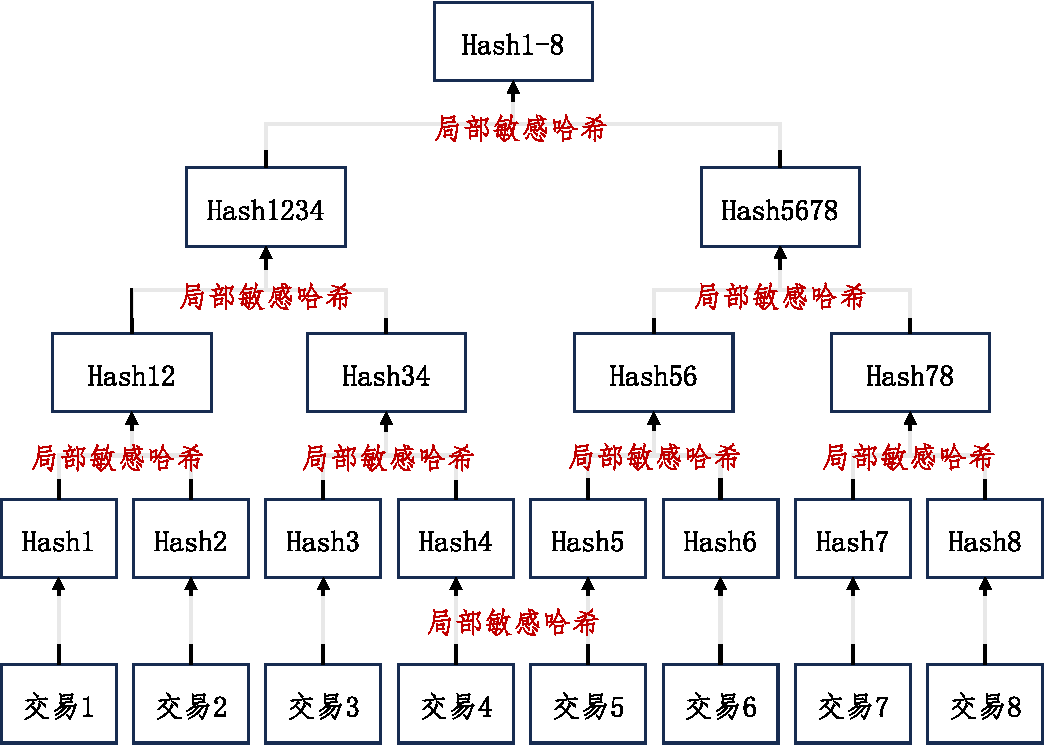
\includegraphics[width=0.85\linewidth]{figures/timechain/lsh_constructure.pdf}
    \caption{LSH树的结构}
    \label{fig:lsh_tree}
\end{figure}

深入分析物联网数据的特性后,本文注意到物联网数据的变化通常较为缓慢,短期内不太可能发生剧烈变动。
针对这些高度相似的数据点,LSH算法能够从相似的原始数据中产生相似的哈希结果。
LSH算法的这一特性保证了即使在哈希处理之后,相似的物联网数据点仍然保持相似性。
基于这一观察,本文设计了一种创新的基于LSH树的验证机制,它采用LSH算法替代了传统默克尔树中使用的通用哈希函数,如\autoref{fig:lsh_tree}所示。
通过仅传输LSH哈希值的差异部分,本文能够显著减少在验证过程中需要传输的数据量,从而提高了数据传输的效率。

本文在\autoref{fig:tail_merging_lsh}中展示了LSH树的一个具体例子。
具体来说,对于批处理中的数据,本文采取类似于默克尔树的步骤,首先对原始数据执行局部敏感哈希。
在叶子层,对于相似的原始数据$0...000$和$0...001$,他们的哈希结果也是类似的,分别是\texttt{d...eac}和\texttt{d...ead}。
因此,在传输第一级哈希值时,TimeChain只需要最后一位哈希值即可。
针对这两个相似的哈希值,TimeChain也对其做局部敏感哈希,得到的结果与另一组原始数据的哈希值相似,这也可以极大地减少需要传输的哈希位数。
然后,TimeChain逐层向上重复这个过程,直到得到一个唯一的哈希值,即哈希根。
通过类比,对于每一层的哈希值,TimeChain只需要传输差分的哈希比特,从而进一步减少了传输的数据量。

\section{LSH树的尾部合并机制}

\begin{figure}[t]
    \centering
	\begin{minipage}{0.8\linewidth}
        \centering
        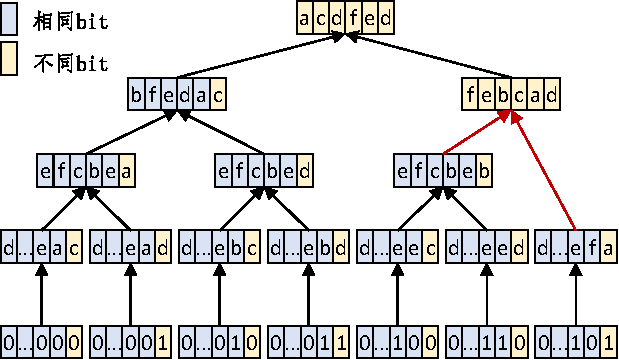
\includegraphics[width=1\textwidth]{figures/timechain/tail_merging_lsh.pdf}
        \caption{非满二叉LSH树}
        \label{fig:tail_merging_lsh}
	\end{minipage}
\end{figure}

在一个完整的二叉树中,LSH树可以通过成对地批量合并数据来执行局部敏感哈希。
然而,如果批处理中的数据数量不足以形成完整的二叉树,那么像默克尔树一样构建哈希树将导致相似性的丧失。
在\autoref{fig:tail_merging_lsh}中,一批中有7个数据点,这并不足以形成一棵满二叉树。
在第一轮哈希中,前6个数据成对执行LSH。
由于原始数据的相似性,这6个数据的哈希结果是相似的。
在第二轮哈希中,由于数据5-6和第7个原始数据的第一轮哈希结果非常不同,这两个数据的哈希结果也与数据点1-4的哈希结果非常不一样。
在执行完整性证明时,需要传输所有这些不同的哈希数据位,这增加了传输的数据量。

\begin{figure}[t]
    \centering
	\begin{minipage}{0.8\linewidth}
        \centering
        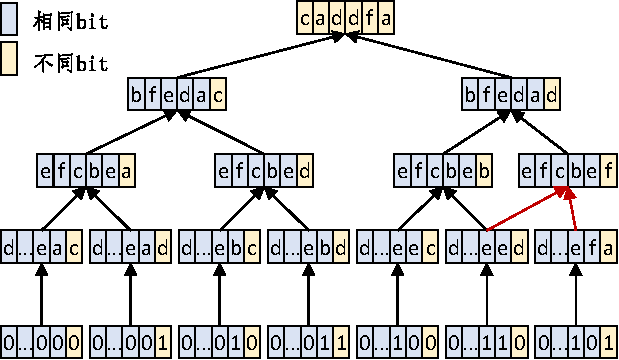
\includegraphics[width=1\textwidth]{figures/timechain/tail_merging_tail.pdf}
	\end{minipage}
	\caption{尾部合并下的非满二叉LSH树}
	\label{fig:tail_merging_tail}
\end{figure}
为了解决这个问题,本文引入了尾部合并策略,将非全二叉树的尾部节点与同一层的前节点合并。
如\autoref{fig:tail_merging_tail}所示,在第一轮哈希中,本文将第7个节点和第6个节点合并,以尽可能保持数据的相似性。
数据6-7的哈希结果是\texttt{efcbeb},数据5-6的哈希值是\texttt{efcbef}。
显然,在第一轮哈希中存在很高的相似性,并且可以保持到下一级哈希。
这将传输的哈希值大小从12位减少到7位,代价是在第一轮哈希中只传输了1个不同的比特。
这样,在进行完整性证明时,本文只需要传输不同的哈希位,从而减少了传输的数据量。

\section{LSH树的安全性分析}
鉴于本文提出的解决方案中采用了LSH树替代了传统的默克尔树,对LSH树的安全性进行深入分析变得至关重要。
LSH树的设计初衷是为了减少数据传输量,同时保持数据验证的准确性。
然而,这种替代可能会引入新的安全风险。
本文主要关注数据篡改问题,即在LSH树结构中,存储提供者是否能够通过改变数据内容来得到与未篡改数据相同的哈希值。
为了评估这一风险,本文对LSH树的不同层级进行了广泛的测试,以确定在何种程度上篡改数据而不被检测到是可行的。

测试结果表明,在最接近数据源的哈希层,也就是LSH树的最底层,哈希值的平均差位数达到了170位。
这一数值远超过了广泛使用的MD5和SHA1哈希算法的安全性标准,这些标准现在在物联网场景中非常常用~\cite{chi2017hashing,landge2018secured}。
因此,LSH树在底层提供的170位的哈希差位数,为数据完整性提供了更强的安全保障。

对于LSH树靠近根节点的高层级,虽然哈希差位数较少,但这并不意味着篡改数据变得容易。
实际上,由于LSH树的结构特性,即使是高层级的少量哈希差异也足以被检测出来,因为这些差异会随着树的结构向上传播,最终影响到根哈希值。
因此,任何对原始数据的篡改,无论在树的哪一层,都很难不被察觉。

综上所述,LSH树不仅提供了与传统默克尔树相似的数据验证功能,而且在安全性方面仍然符合物联网场景的需要。

\section{本章小结}
本章针对物联网数据完整性验证过程中的数据传输延迟问题,提出了一种基于LSH树的新型验证机制。
本章发现,在传输的数据中,数据完整性证明占据了相当大的比例,且通常以默克尔树的形式组织,这导致为了验证数据完整性需要传输的数据量几乎是原始数据量的两倍。
为了解决这一问题,本章利用物联网数据变化缓慢且高度相似的特性,采用LSH算法替代了传统默克尔树中的通用哈希函数,通过仅传输LSH哈希值的差异部分,显著减少了验证过程中需要传输的数据量。

本章详细分析了LSH树的结构和工作流程,并针对非满二叉树的情况,引入了尾部合并策略以保持数据的相似性,进一步减少了传输的数据量。
此外,本章还对LSH树的安全性进行了分析,确保了其在最接近数据源的哈希层中具有足够的安全性,超过了现有的MD5和SHA1标准,在物联网场景中足够安全。
